\documentclass{article}
\usepackage[utf8]{inputenc}
\usepackage[english]{babel}

\usepackage{geometry}
\geometry{letterpaper,margin=1in}
\usepackage{graphicx}
\usepackage{enumitem}
\usepackage{amssymb}
\usepackage{amsmath}
\usepackage[all]{xy}
\usepackage{hyperref}
\usepackage{mathabx}
\usepackage{tikz}
\usepackage{mathabx}
\usepackage[]{amsthm} %lets us use \begin{proof}
\DeclareGraphicsRule{.tif}{pnf}{.png}{'convert #1 'dirname #1'/'basename #1.tif'.png}

\newcommand{\bigzero}{\mbox{\normalfont\Large\bfseries 0}}

\usepackage{subfig}

\usepackage{rotating}
\usepackage{tabularx}
\usepackage{caption}
\usepackage{xspace}

\newcommand{\Rbb}{\mathbb{R}}
\newcommand{\Pbb}{\mathbb{P}}


\setlength\parindent{0pt}

\begin{document}
\theoremstyle{definition}
\newtheorem{theorem}{Theorem}[section]
\theoremstyle{definition}
\newtheorem{conjecture}[theorem]{Conjecture}
\theoremstyle{definition}
\newtheorem{definition}[theorem]{Definition}
\theoremstyle{definition}
\newtheorem{goal}[theorem]{Goal}
\theoremstyle{definition}
\newtheorem{corollary}[theorem]{Corollary}
\theoremstyle{definition}
\newtheorem{question}[theorem]{Question}
\theoremstyle{definition}
\newtheorem{lemma}[theorem]{Lemma}
\theoremstyle{definition}
\newtheorem{proposition}[theorem]{Proposition}

\section{$\Delta(\Rbb)$ being Empty implies $Y(\Rbb)$ is Connected}

\begin{lemma}
$\pi_2(\Rbb)(Y(\Rbb)) = \{p \in \Pbb^2_{[u:v:w]}(\Rbb)\ |\ Q_1(p) \geq 0 \text{ or } \Delta(p) \leq 0\}$
\end{lemma}

\begin{proposition}
If the topological type of $\Delta(\Rbb)$ is empty, then $Y(\Rbb)$ is Connected.
\end{proposition}

\begin{proof}
It suffices for us to show that $\pi_2(\Rbb)(Y(\Rbb))$ is connected, since every fiber of the image is connected and $\pi_2$ is a close map.\\\\
Since $\Delta(\Rbb)$ is empty, $\Delta$ has no real roots, so either $\Delta > 0$ or $\Delta < 0$ for all $p \in \Pbb^2_{[u;v;w]}(\Rbb)$.\\\\
If $\Delta < 0$, then from Lemma 1.1 $\pi_2(\Rbb)(Y(\Rbb)) = \Pbb^2_{[u;v;w]}(\Rbb)$ is connected.\\\\
If $\Delta > 0$, then $\pi_2(\Rbb)(Y(\Rbb)) = (Q_1 \geq 0)$.\\\\
If $Q_1$ is positive definite, then $\pi_2(\Rbb)$ is again surjective. If $Q_1$ is negative definite, then $\pi_2(\Rbb)(Y(\Rbb)) = \O$, so $Y(\Rbb) = \O$ is connected. If $Q_1$ is indefinite, then $(Q_1 \geq 0)$ is either an oval or the complement of an oval, which are both connected.
\end{proof}

\section{$\Delta(\Rbb)$ being One Oval implies $Y(\Rbb)$ is Connected}

\begin{proposition}
If the topological type of $\Delta(\Rbb)$ is one oval, then $Y(\Rbb)$ is connected.
\end{proposition}

\begin{proof}
It suffices for us to show that $\pi_2(\Rbb)(Y(\Rbb))$ is connected, since every fiber of the image is connected and $\pi_2$ is a close map.\\\\
If $Q_1$ is positive definite, then $\pi_2(\Rbb)(Y(\Rbb)) = \Pbb^2_{[u:v:w]}(\Rbb)$ is connected.\\\\
If $Q_1$ is negative definite, then $\pi_2(\Rbb)(Y(\Rbb)) = \{p \in \Pbb^2_{[u:v:w]}(\Rbb)\ | \Delta(p) \leq 0\}$, which is connected since $\Delta(\Rbb)$ is one oval, so both $\Delta(\Rbb)$ and its complement is connected.\\\\
If $Q_1$ is indefinite, assume for the sake of contradiction that $Y(\Rbb)$ is disconnected, since $(Q_1 \geq 0)$ and $(\Delta(p) \leq 0)$ are both connected, it has to be the case that $\pi_2(Y(\Rbb))$ has 2 connected components being $(Q_1 \geq 0)$ and $(\Delta(p) \leq 0)$.\\\\
But we note that for all $p \in (Q_1 = 0)$, we have that $\Delta(p) = -Q_2(p) \leq 0$, so $(Q_1 = 0)$ is contained in $(\Delta(p) \leq 0)$. But this means that $\pi_2(Y(\Rbb))$ is clearly connected. So we have a contradiction.\\\\
Thus, in all cases, $Y(\Rbb)$ is connected.
\end{proof}

\section{$\Delta(\Rbb)$ being Four Ovals implies $Y(\Rbb)$ is Connected}

\begin{lemma}
Let $f: X \to Y$ be a quotient map and the fiber of every point in $Y$ is connected. Then for each connected open or closed subset $U \subset Y$, $f^{-1}(U)$ is connected in $X$.
\end{lemma}

\begin{proof}
Since $f^{-1}(U)$ is open/closed and saturated, the restriction of $f$ onto $f^{-1}(U)$ gives a quotient map $f': f^{-1}(U) \to U$. Since $f'$ is a quotient map with connected base and every fiber is connected, $f^{-1}(U)$ is connected.
\end{proof}

\begin{lemma}
Let $f: X \to Y$ be a close map such that the fiber of every point in $f(X)$ is connected. Suppose $f(X)$ has a finite number of connected components, then $X$ and $f(X)$ has the same number of connected components.
\end{lemma}

\begin{proof}
We can without loss take $Y = f(X)$ and just consider $f$ to be surjective. Let $m$, $n$ be the number of connected components in $X$ and $Y$ respectively. We first note that clearly $m \geq n$ since the continuous image of a connected set is connected.\\\\
Now for each connected component $C_i, 1 < i < n$ in $f(X)$, $C_i$ is closed, so $f^{-1}(C_i)$ is also connected in $X$ by Lemma 3.1. The union of all $f^{-1}(C_i)$ is $X$, so $X$ has at most $n$ connected components, so $m \leq n$.\\\\
Thus, we have that $m = n$.
\end{proof}

\begin{proposition}
If the topological type of $\Delta(\Rbb)$ is four ovals, then $Y(\Rbb)$ is connected.
\end{proposition}

\begin{proof}
It suffices for us to show that $\pi_2(\Rbb)(Y(\Rbb))$ is connected, since every fiber of the image is connected and $\pi_2$ is a close map.\\\\
If $Q_1$ is positive definite, then $\pi_2(\Rbb)(Y(\Rbb)) = \Pbb^2_{[u:v:w]}(\Rbb)$ is connected.\\\\
If $Q_1$ is negative definite, then $\pi_2(\Rbb)(Y(\Rbb)) = (\Delta \leq 0)$ is either 4 ovals or the complement of four ovals. The latter case is a connected image, so suppose $\pi_2(\Rbb)(Y(\Rbb))$ is 4 ovals, then it has 4 connected components.\\\\
Then Lemma 3.2 tells us that $Y(\Rbb)$ has $4$ connected components, but this also means that $\pi_1(Y(\Rbb))$ has 4 connected components. But this would imply that $det(M_1t_0^2 + 2M_2t_0t_1 + M_3t_1^2)$ has at least $8$ roots in $\Pbb^1_{[t_0:t_1]}(\Rbb)$, which is impossible since it can only have at most $6$ roots.\\\\
If $Q_1$ is indefinite, then we first note that for all $p \in (Q_1 = 0)$, $\Delta(p) = -Q_2(p)^2 \leq 0$, so we have that $(Q_1 = 0) \subset (\Delta \leq 0)$.\\\\
If $(\Delta \leq 0)$ is the complement of 4 ovals, then $(\Delta \leq 0)$ itself is already connected, and we know that $(Q_1 \geq 0)$ is also connected. Since the union of two connected sets with non-empty intersection is connected, we have that $\pi_2(\Rbb)(Y(\Rbb)) = (\Delta \leq 0) \cup (Q_1 \geq 0)$ is connected.\\\\
If $(\Delta \leq 0)$ is 4 ovals, then since $(Q_1 = 0)$ is connected, $(Q_1 = 0)$ has to be contained in only 1 of the 4 ovals.\\\\
Now if $(Q_1 \geq 0)$ is an oval, then $(Q_1 \geq 0) \subset (\Delta \leq 0)$, so $\pi_2(\Rbb)(Y(\Rbb)) = (\Delta \leq 0)$ is 4 ovals. Then using Lemma 3.2 again leads to a contradiction.\\\\
If $(Q_1 \geq 0)$ is the complement of an oval, then $\pi_2(\Rbb)(Y(\Rbb)) = \Pbb^2(\Rbb)$, so the image is connected.
\end{proof}

\section{Topological Type of $\Delta(\Rbb)$ and Number of Connected Components}

\begin{lemma}
If $(\Delta \leq 0)$ is connected, then $Y(\Rbb)$ is connected.
\end{lemma}

\begin{proof}
We already know that $(Q_1 = 0) \subset (\Delta \leq 0)$ and $\pi_2(\Rbb)(Y(\Rbb)) = (\Delta \leq 0) \cup (Q_1 \geq 0)$. Since both $(\Delta \leq 0)$ and $(Q_1 \geq 0)$ are connected and they have non-empty intersection, $\pi_2(\Rbb)(Y(\Rbb))$ is connected.\\\\
Since $\pi_2$ is closed and the fiber of every point in its image is connected, we have that $Y(\Rbb)$ is connected.
\end{proof}

\begin{proposition}
If $\pi_1(Y(\Rbb))$ has $3$ connected components, then the topological type of $\Delta(\Rbb)$ is 3 ovals.
\end{proposition}

\begin{proof}
From Proposition 1.2, 2.1, and 3.3, we know that $Y(\Rbb)$ can only be disconnected if $\Delta(\Rbb)$ is either 2 non-nested ovals, 2 nested ovals, or 3 ovals. We first note by Lemma 3.2 we know that $\pi_2(Y(\Rbb))$ also needs to have 3 connected components.\\\\
Suppose $\Delta(\Rbb)$ is 2 non-nested ovals. If $(\Delta \leq 0)$ is the complement of two ovals, then it's connected, so Lemma 4.1 tells us that $Y(\Rbb)$ is connected, so we have a contradiction.\\\\
If $(\Delta \leq 0)$ is two ovals, then we know $(Q_1 = 0)$ is contained in one of the two ovals. If $(Q_1 \geq 0)$ is an oval, then $\pi_2(Y(\Rbb))$ has only 2 connected components, hence a contradiction. If $(Q_1 \geq 0)$ is the complement of an oval, then $\pi_2$ is surjective, so $Y(\Rbb)$ is connected.\\\\
Thus, we conclude that $(\Delta \leq 0)$ cannot be 2 non-nested ovals.\\\\
Now suppose $\Delta(\Rbb)$ is instead 2 nested ovals, then there are two cases for $(\Delta \leq 0)$:
\[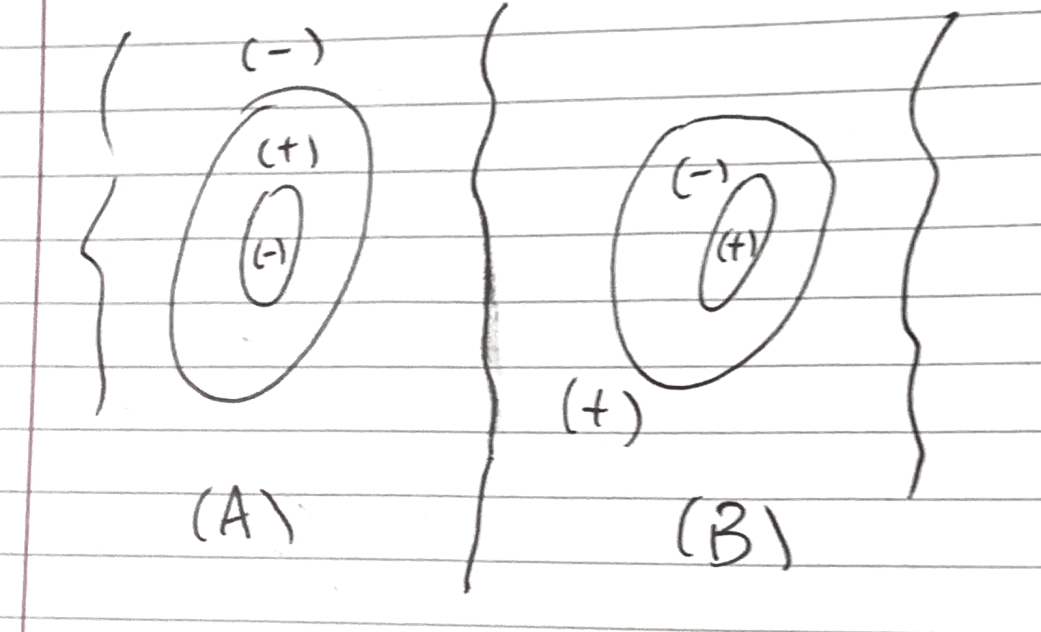
\includegraphics[width=7.5cm]{two_oval_sign.png}\]
Now recall that $(Q_1 = 0)$ is contained in $(\Delta \leq 0)$ and $(Q_1 \geq 0)$ is an oval, then in both Case (A) or (B), it's impossible to turn $\pi_2(Y(\Rbb))$ to have 3 connected components. Thus, we have a contradiction.
\end{proof}


\begin{proposition}
If $\pi_1(Y(\Rbb))$ has $2$ connected components, then the topological type of $\Delta(\Rbb)$ is either $2$ nested ovals or $2$ non-nested ovals.
\end{proposition}

\begin{proof}
It suffices for us to show that $\Delta(\Rbb)$ cannot have the topological type of $3$ ovals. Indeed, Lemma 3.2 tells us that since $\pi_1(Y(\Rbb))$ has $2$ connected components, $\pi_2(Y(\Rbb))$ also has $2$ connected components.\\\\
Now assume for the sake of contradiction that $\Delta(\Rbb)$ has 3 ovals. Now if $(\Delta \leq 0)$ is the complement of 3 ovals, then it's connected, then Lemma 3.1 leads to a contradiction.\\\\
Now if $(\Delta \leq 0)$ is 3 ovals, then $(Q_1 = 0)$ is contained in exactly one oval. If $(Q_1 \geq 0)$ is also an oval, then $\pi_2(Y(\Rbb))$ has 3 connected components, hence a contradiction. If $(Q_1 \geq 0)$ is the complement of an oval, then $\pi_2$ is surjective, which means $Y(\Rbb)$ is connected, hence a contradiction.
\end{proof}

\end{document}
